\begin{frame}[t,fragile]{What is C++?}
\begin{itemize}
  \item \textmark{``C++ is a lightweight abstractions programming language''} (B. Stroustrup).
  
  \mode<presentation>{\vfill\pause}
  \item Continuously evolving since 1983, with a new standard every 3 years since 2011.
    \begin{itemize}
      \item Many compatibility elements.
        \begin{itemize}
          \item Some of them tracing back to 1972.
        \end{itemize}
      \item Evolving a language is hard, and breaking compatibility is even harder.
        \begin{itemize}
          \item Billions of lines of code, and millions of developers.
        \end{itemize}
    \end{itemize}

    \mode<presentation>{\vfill\pause}
    \item \textmark{``When someone says ``I want a programming language in which I need only say what I wish done,'' give him a lollipop.''} (A. Perlis).
\end{itemize}
\end{frame}


\begin{frame}[t,fragile]{A brief history of C++}
\begin{itemize}
  \item 1979: \textgood{C with classes}.
  \item 1983: \textgood{C++ 1.0}.
  \item 1989: \textgood{C++ 2.0}.
  \item 1998: \textgood{C++98} $\rightarrow$ \textmark{ISO/IEC 14882:1998}.
  \item 2003: \textgood{C++03} $=$ C++98 with bug fixes.
  \item 2011: \textgood{C++11} $\rightarrow$ \textmark{ISO/IEC 14882:2011}.
  \item 2014: \textgood{C++14} $=$ C++11 with bug fixes and small improvements.
  \item 2017: \textgood{C++17} $\rightarrow$ \textmark{ISO/IEC 14882:2017}.
  \item 2020: \textgood{C++20} $\rightarrow$ \textmark{ISO/IEC 14882:2020}.
  \item 2023: \textgood{C++23} (published 2024) $\rightarrow$ \textmark{ISO/IEC 14882:2024}.
  \item 2026: \textgood{C++26} $\rightarrow$ \textmark{ISO/IEC 14882:2026 (expected)}.
\end{itemize}
\end{frame}

\begin{frame}[t,fragile]{C++98}
\mode<presentation>{\vspace{-1em}} 
\begin{center}
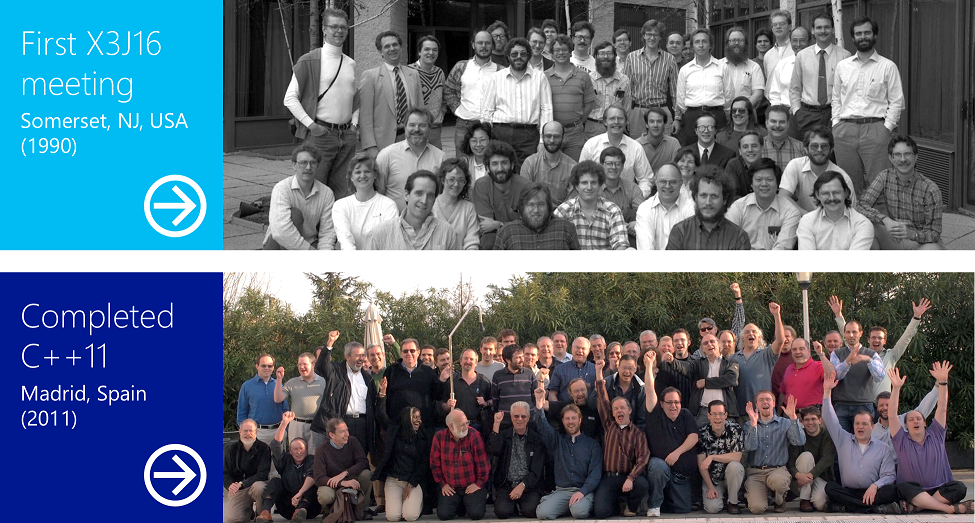
\includegraphics[width=\textwidth]{img/cpp-90-11}
\end{center}
\end{frame}

\begin{frame}[t,fragile]{C++14}
\mode<presentation>{\vspace{-1em}} 
\begin{center}
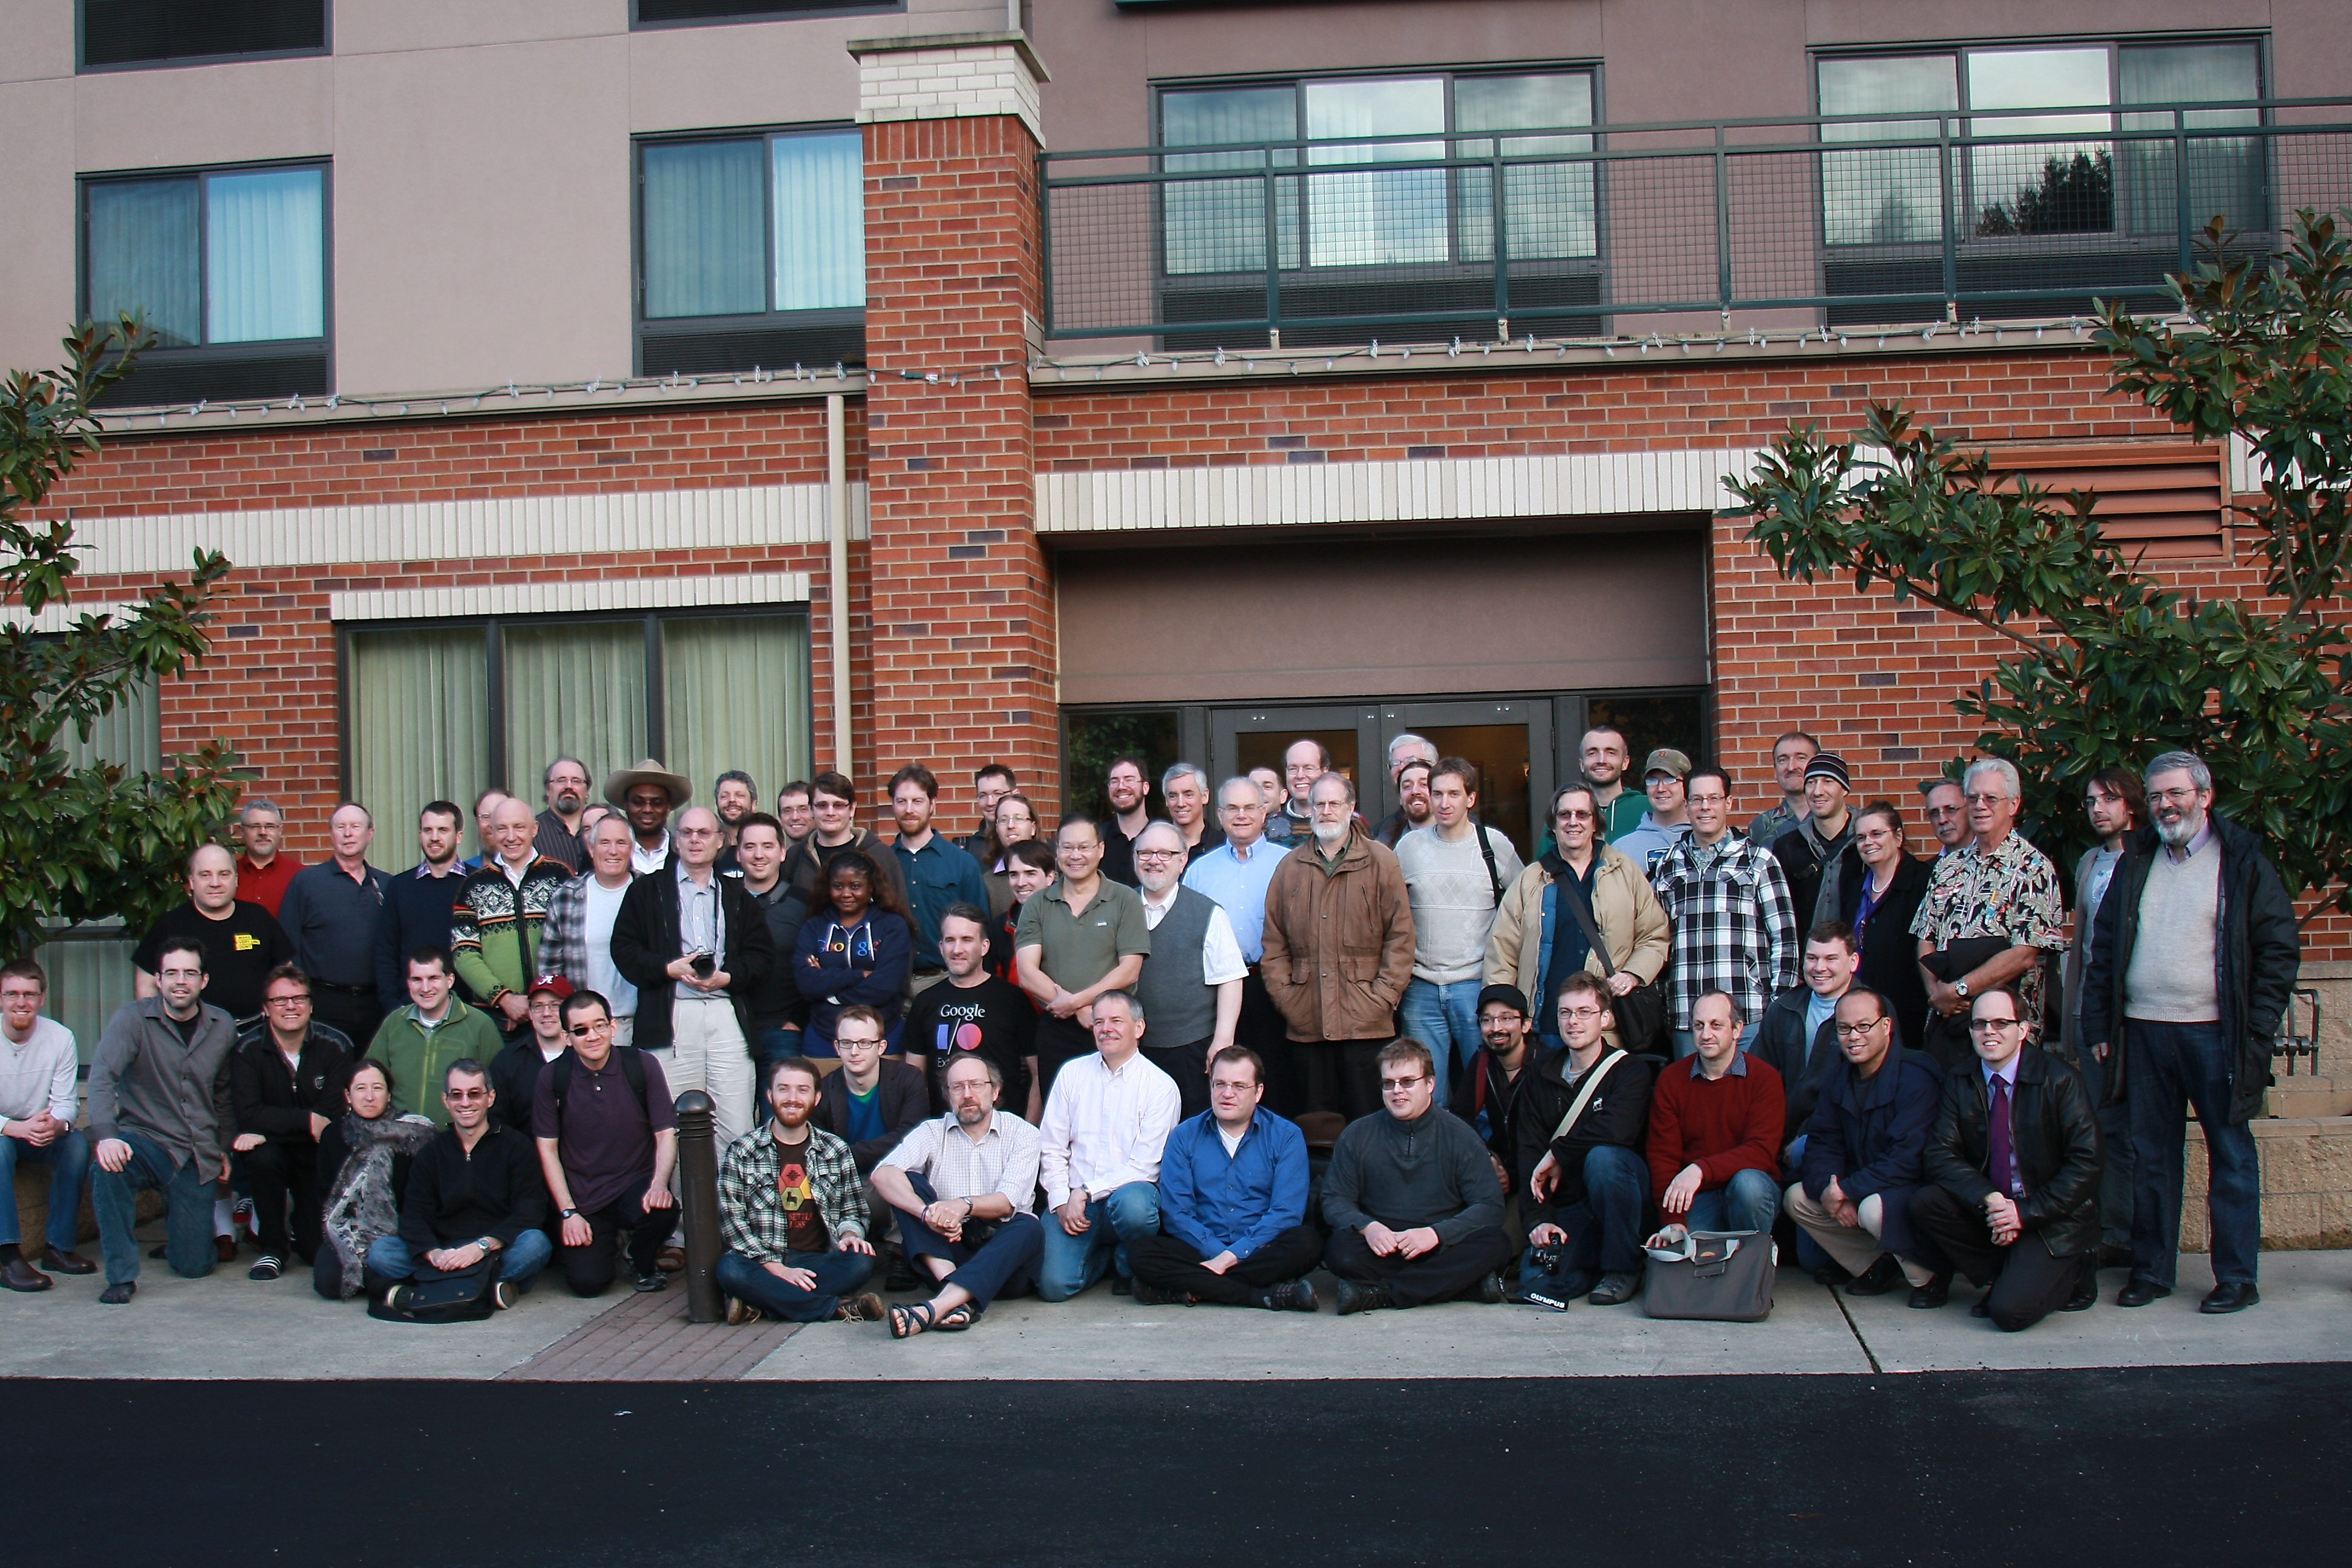
\includegraphics[width=\textwidth]{img/cpp-14}
\end{center}
\end{frame}

\begin{frame}[t,fragile]{C++17}
\mode<presentation>{\vspace{-1em}} 
\begin{center}
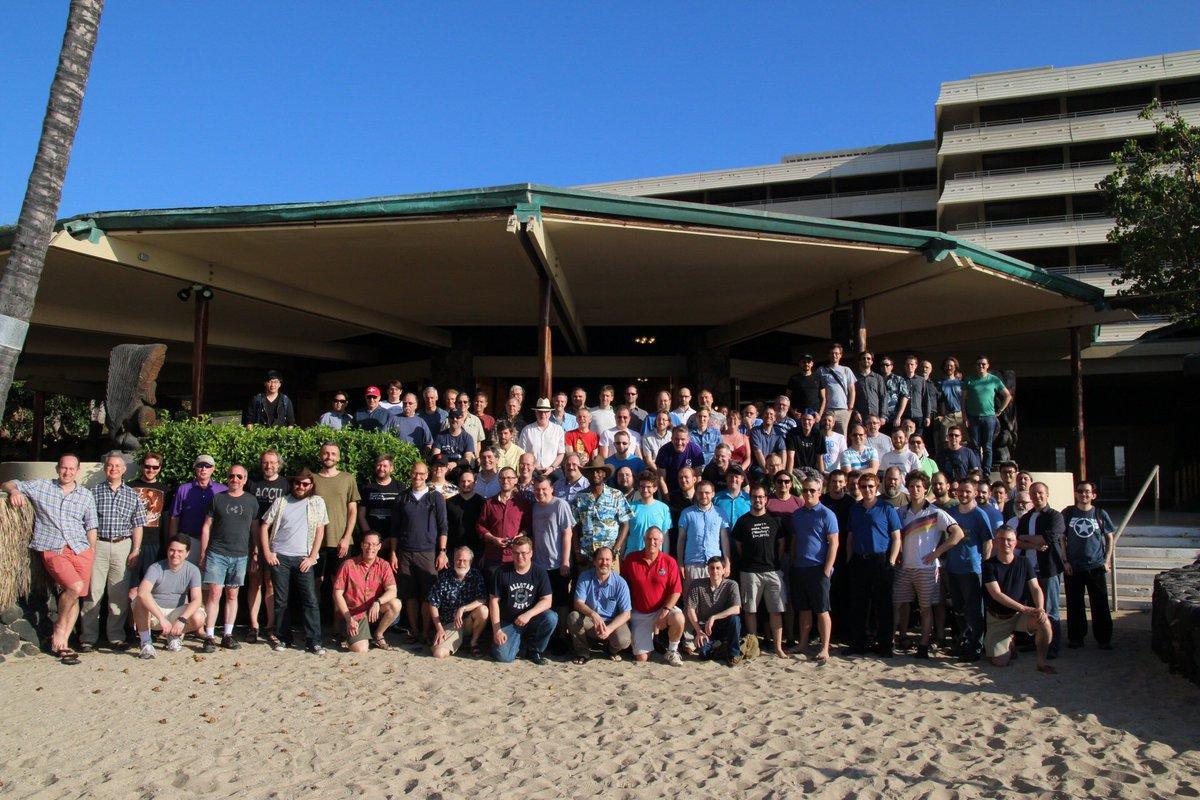
\includegraphics[width=\textwidth]{img/cpp-17}
\end{center}
\end{frame}

\begin{frame}[t,fragile]{C++20}
\mode<presentation>{\vspace{-1em}}
\begin{center}
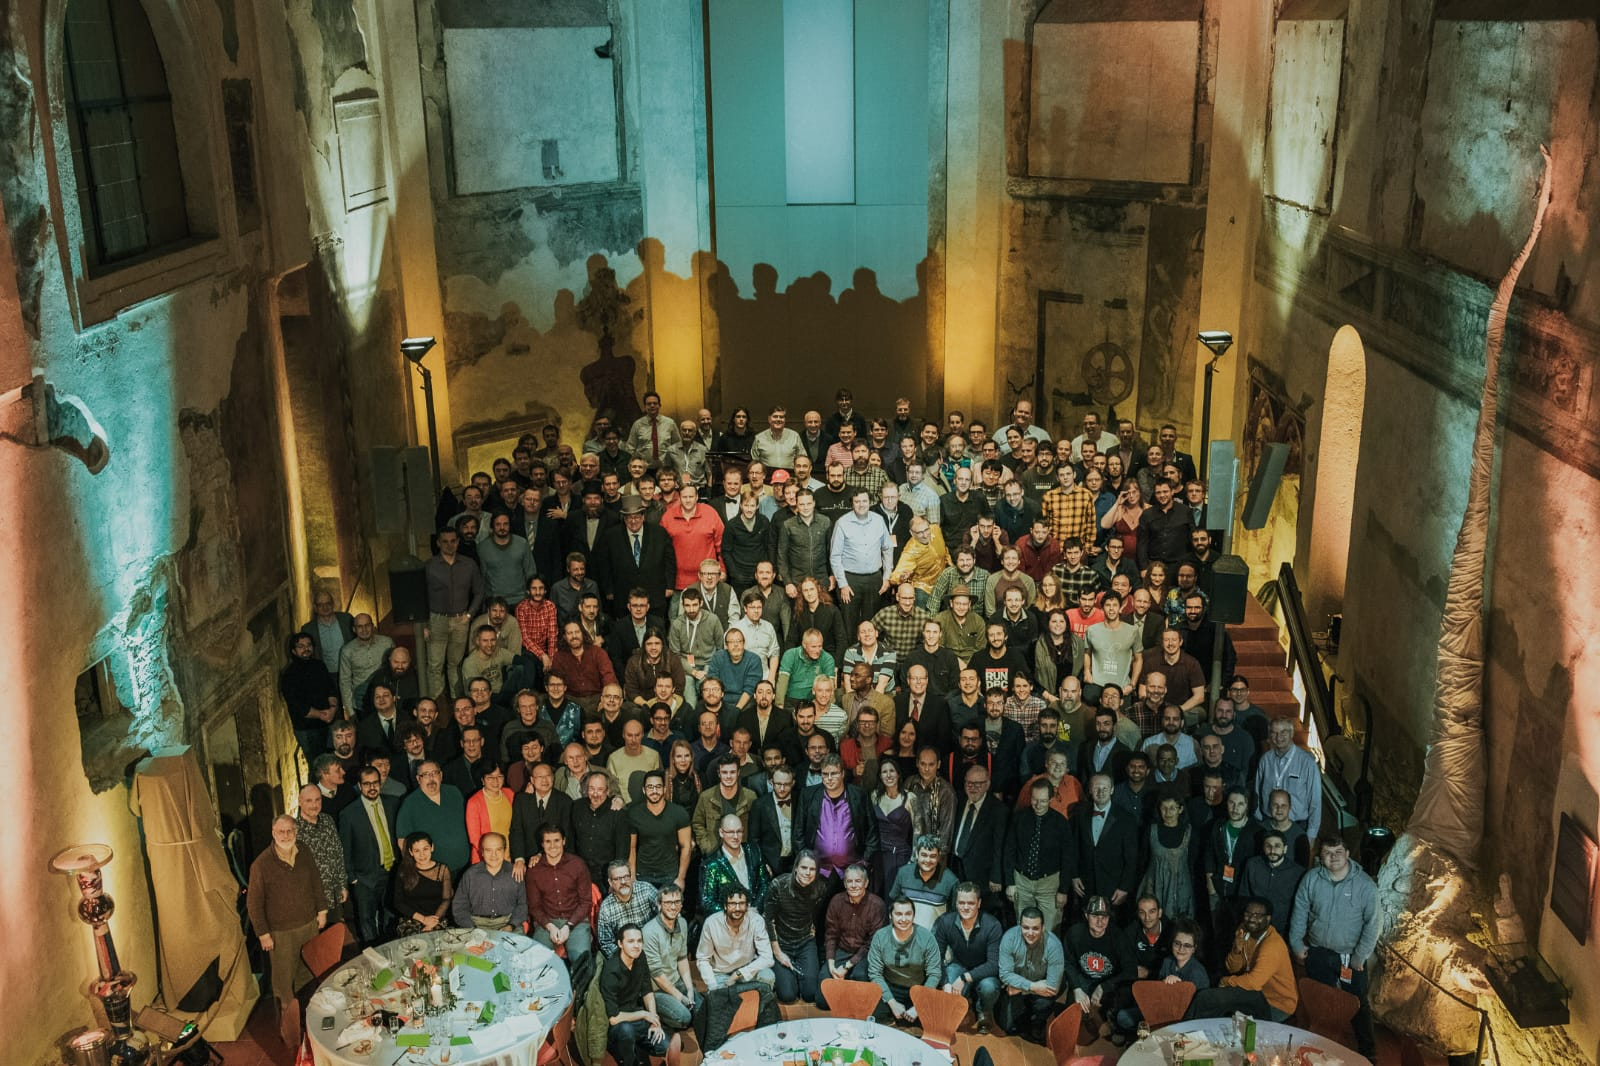
\includegraphics[height=\textheight]{img/cpp-20}
\end{center}
\end{frame}

\begin{frame}[t,fragile]{C++23}
\mode<presentation>{\vspace{-1em}}
\begin{center}
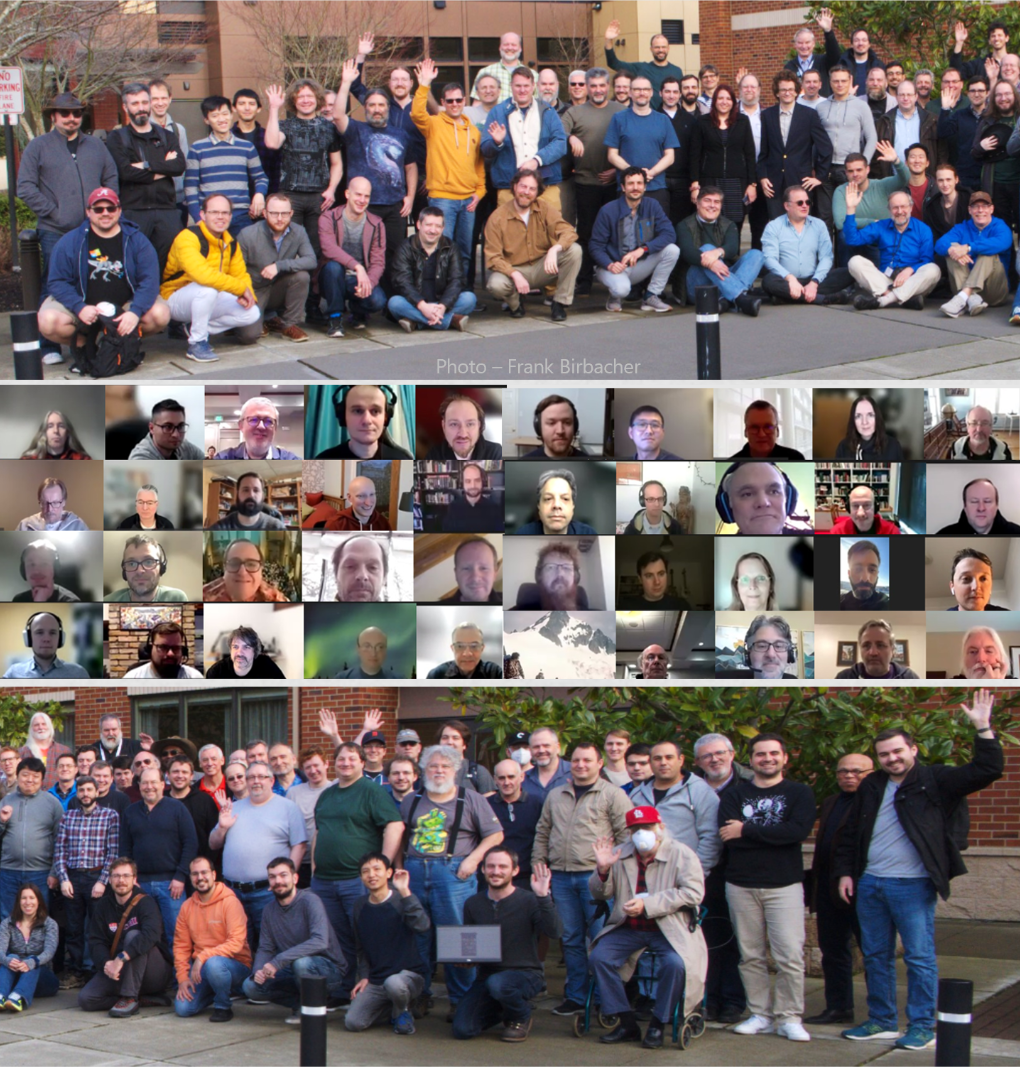
\includegraphics[height=\textheight]{img/cpp-23}
\end{center}
\end{frame}

\begin{frame}[t,fragile]{C++26}
\mode<presentation>{\vspace{-1em}}
\begin{center}
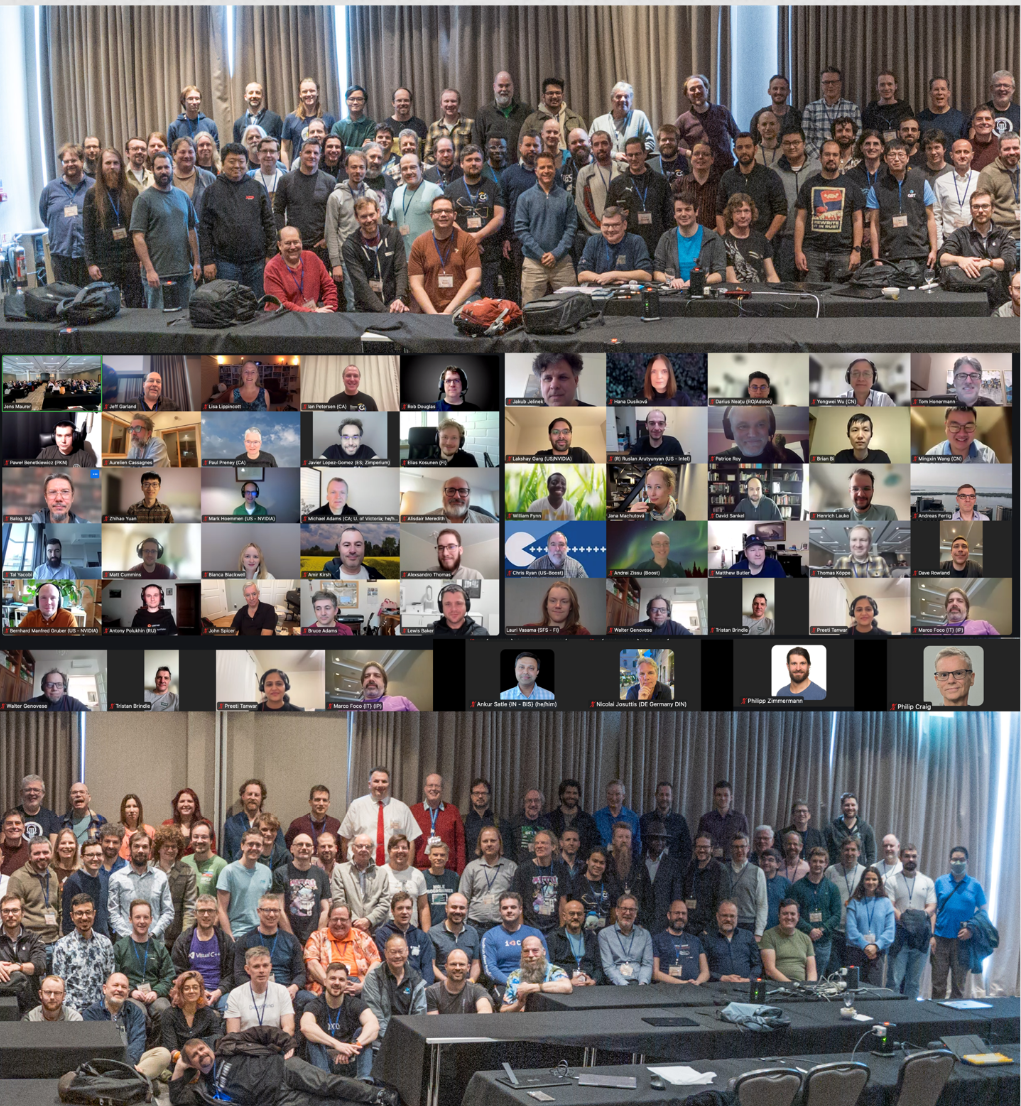
\includegraphics[height=\textheight]{img/cpp-26}
\end{center}
\end{frame}

\begin{frame}[t,fragile]{ISO C++ committee structure}
\mode<presentation>{\vspace{-1em}}
\begin{center}
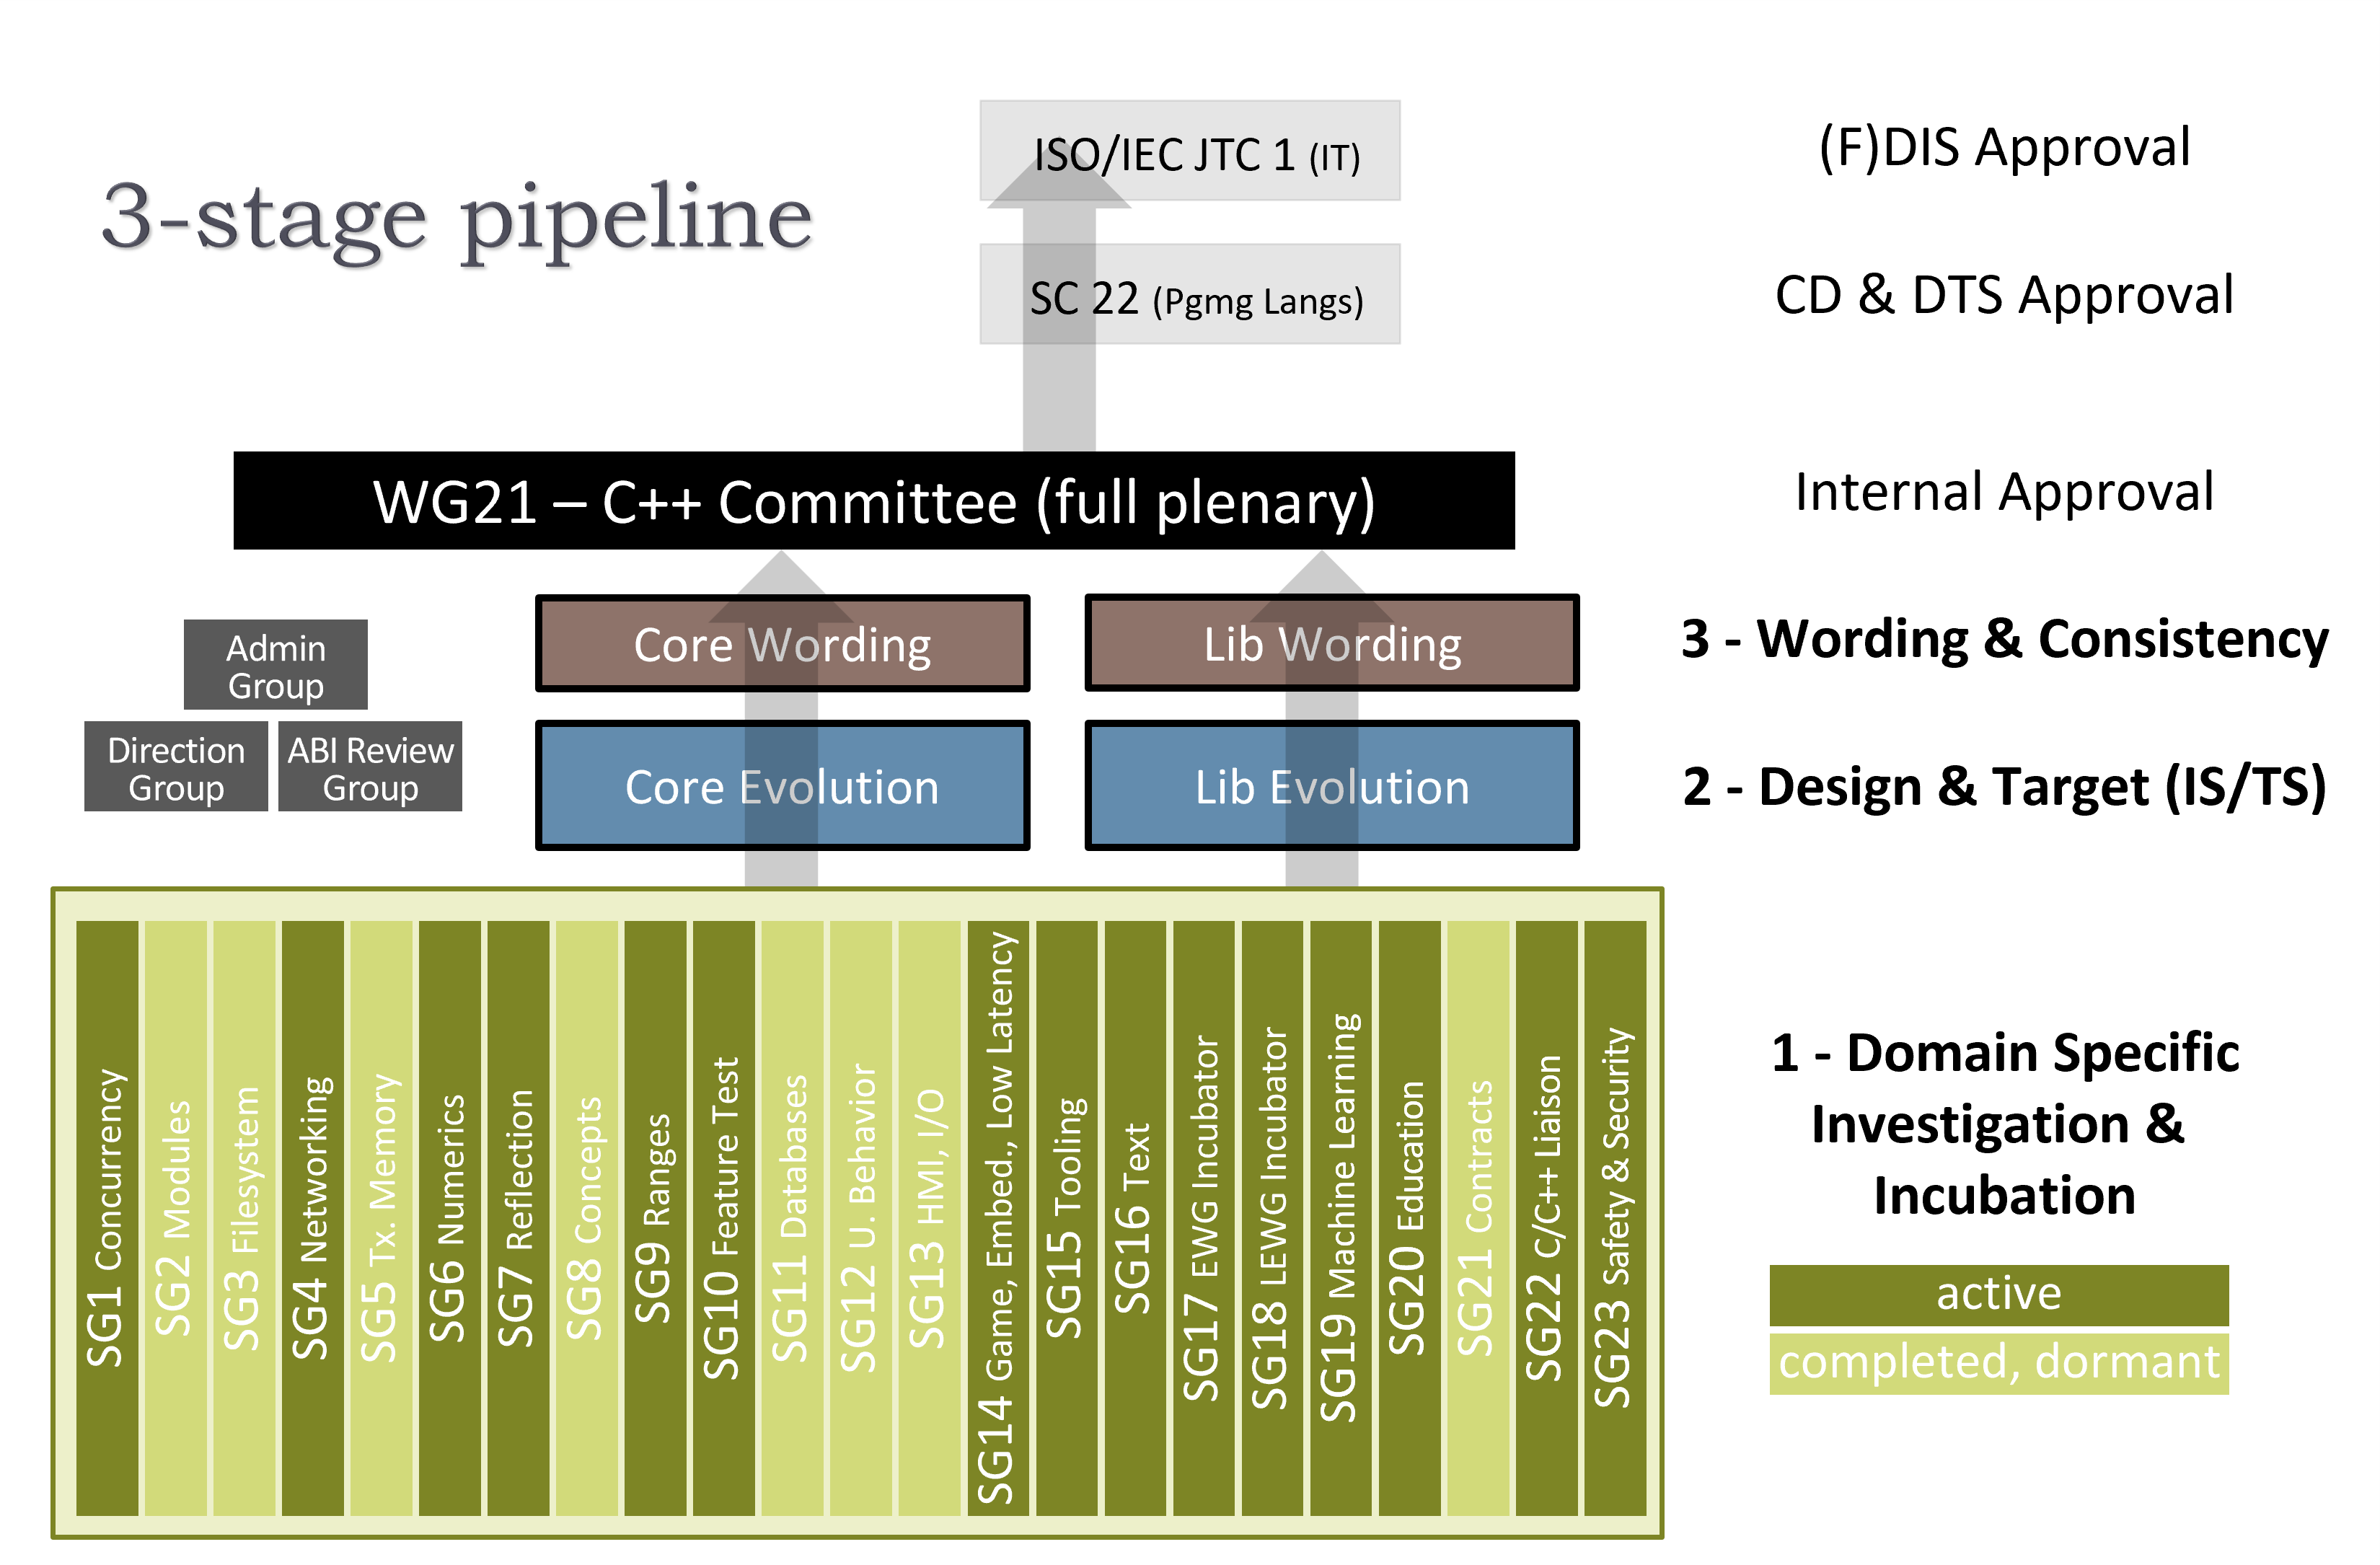
\includegraphics[height=\textheight]{img/wg21-structure}
\end{center}
\end{frame}

\begin{frame}[t,fragile]{ISO C++ timeline}
\mode<presentation>{\vspace{-1em}}
\begin{center}
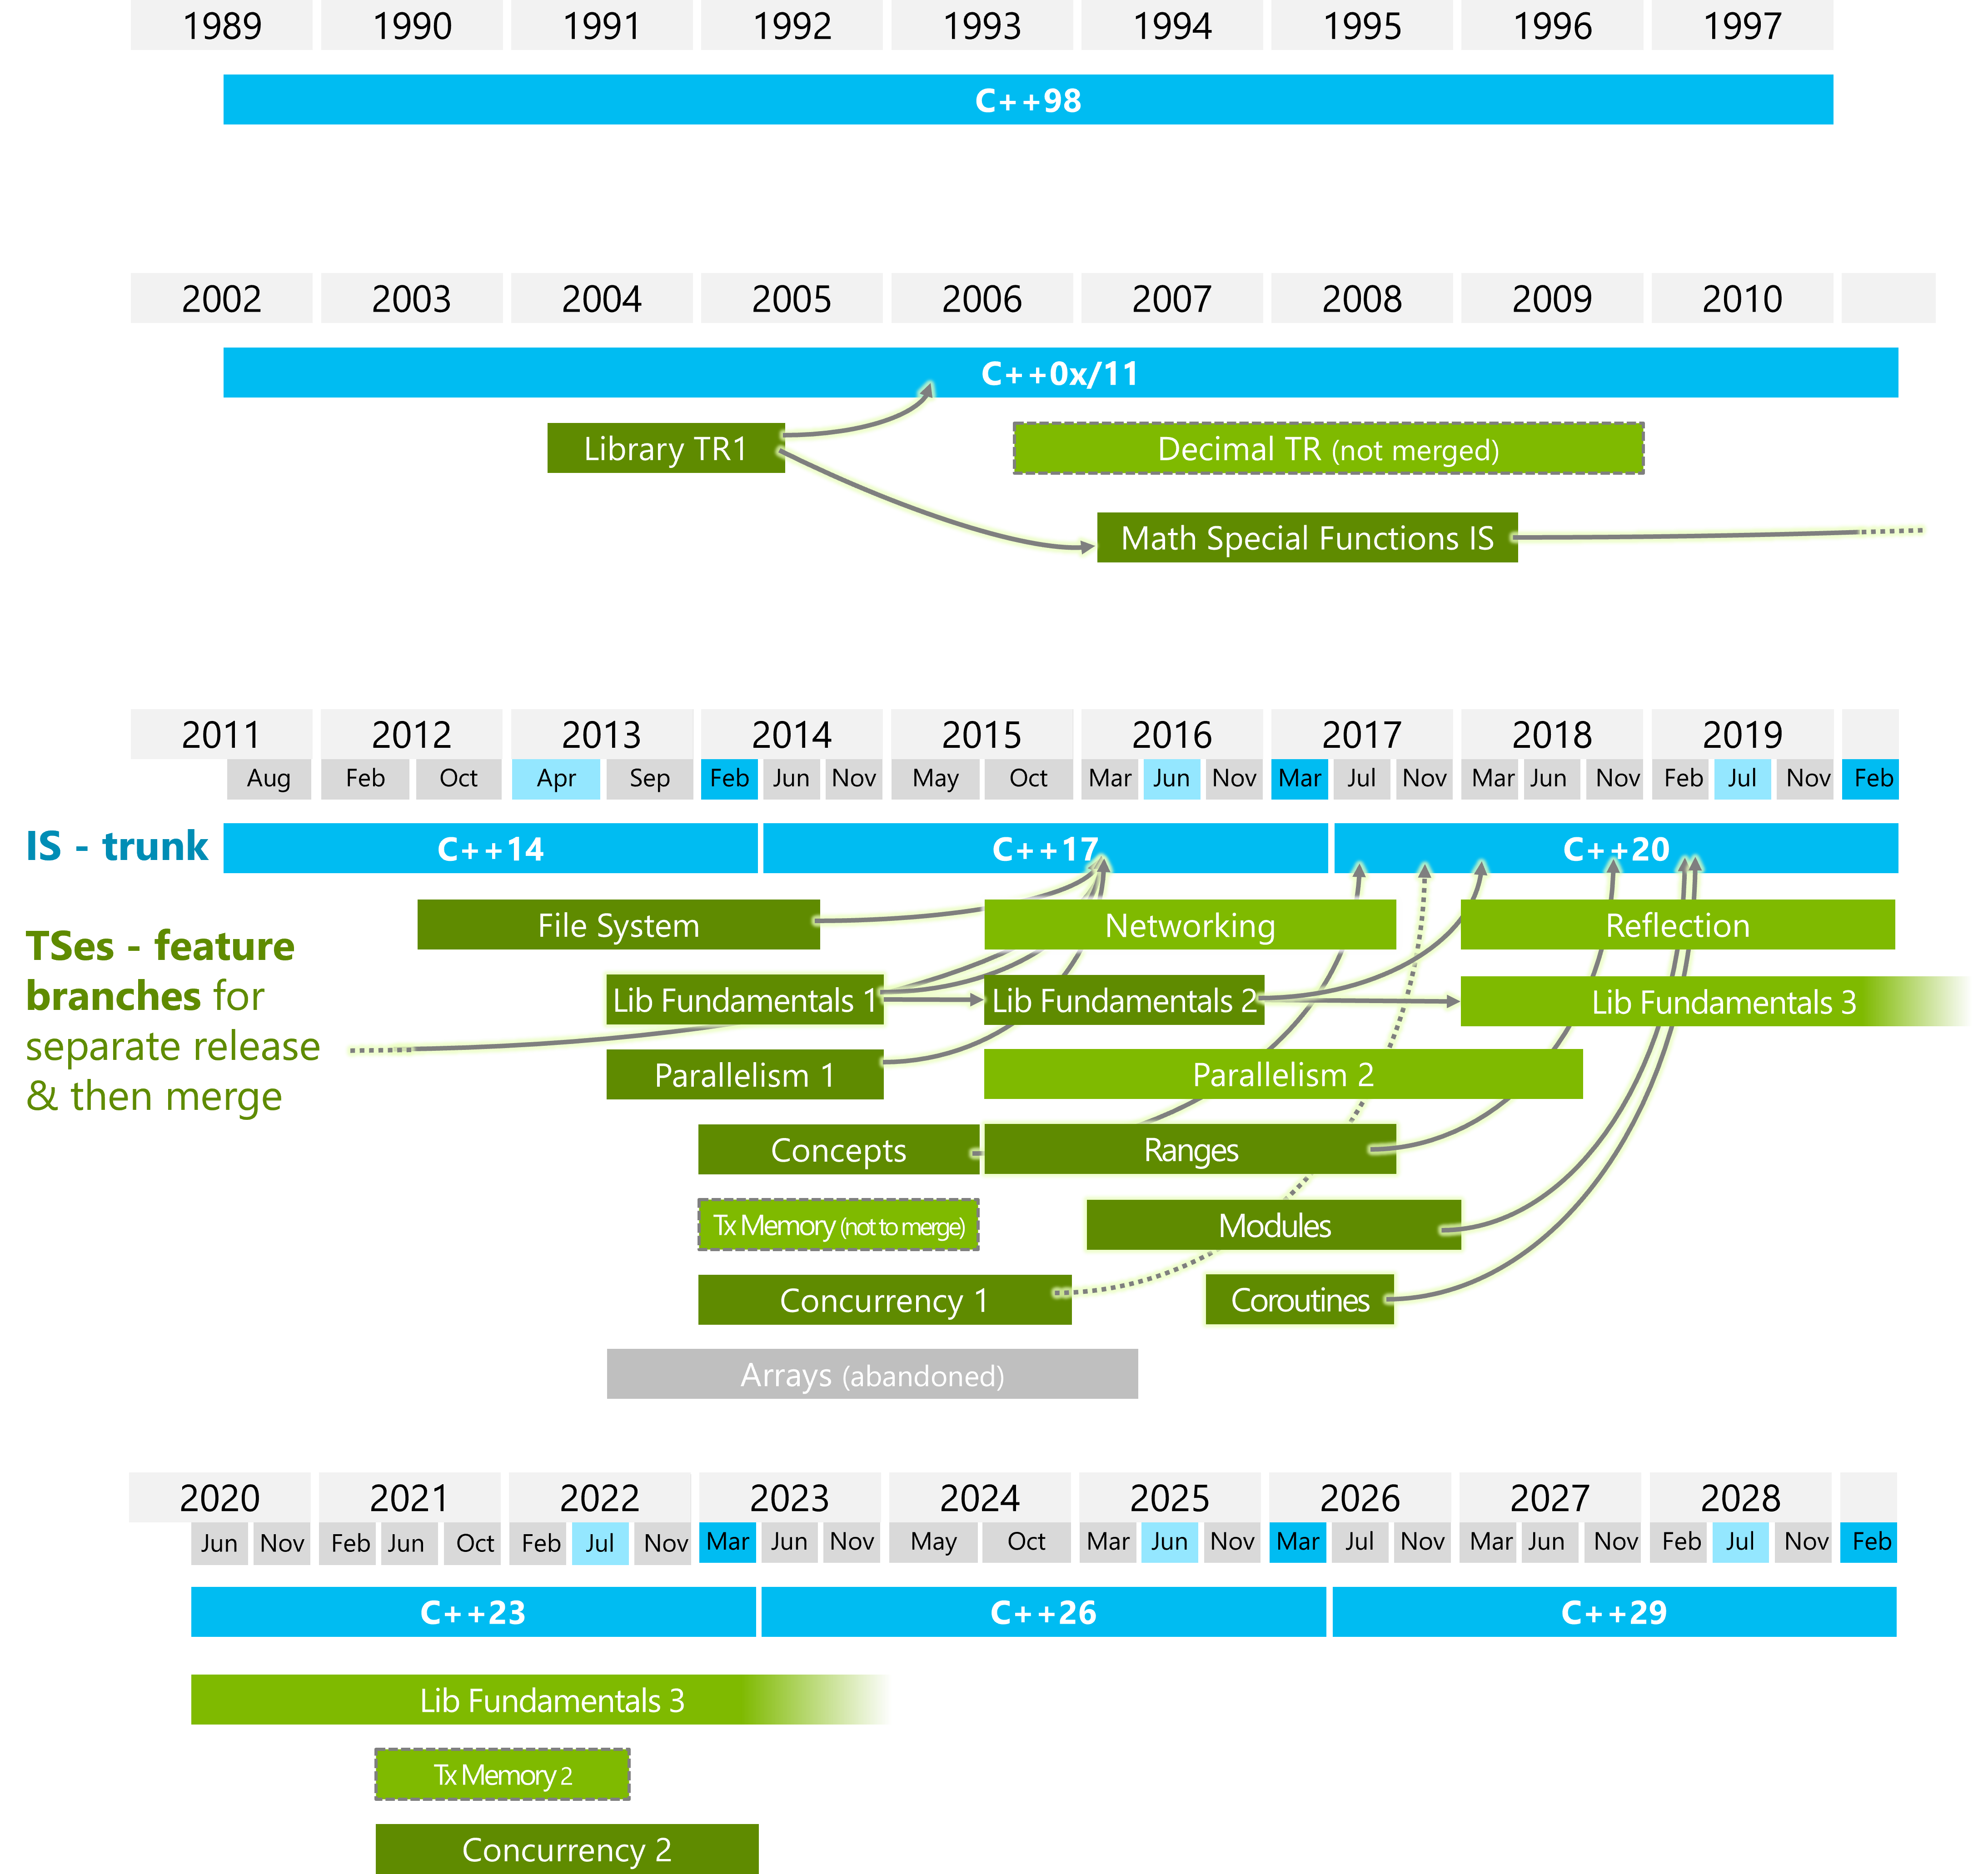
\includegraphics[height=\textheight]{img/wg21-timeline}
\end{center}
\end{frame}

\begin{frame}[t,fragile]{Design principles for C++}
\begin{itemize}
  \item Keep \textmark{backwards compatibility}.
  
  \mode<presentation>{\vfill\pause}
  \item Better to \textmark{extend the library} than the language.
  
  
  \mode<presentation>{\vfill\pause}
  \item Ease the design of \textmark{systems and libraries} (instead of concrete domains).
  
  \mode<presentation>{\vfill\pause}
  \item Improve \textmark{type safety}.
  
  \mode<presentation>{\vfill\pause}
  \item Improve \textmark{performance} and \textmark{interaction with hardware}.
  
  \mode<presentation>{\vfill\pause}
  \item \textmark{Zero-overhead} principle.
  
  \mode<presentation>{\vfill\pause}
  \item Make C++ easier to \textmark{teach and learn}.
\end{itemize}
\end{frame}
